\documentclass{article}
\usepackage[version=3]{mhchem} % Package for chemical equation typesetting
\usepackage{siunitx} % Provides the \SI{}{} and \si{} command for typesetting SI units
\usepackage{graphicx} % Required for the inclusion of images
\usepackage{natbib} % Required to change bibliography style to APA
\usepackage{amsmath} % Required for some math elements 
\usepackage{amsfonts}
\usepackage{listings}
\usepackage{graphicx}
\usepackage[T1]{fontenc}







\setlength\parindent{0pt} % Removes all indentation from paragraphs
\newcommand{\deriv}{\mathrm{d}}
\renewcommand{\labelenumi}{\alph{enumi}.} % Make numbering in the enumerate environment by letter rather than number (e.g. section 6)

%\usepackage{times} % Uncomment to use the Times New Roman font

%----------------------------------------------------------------------------------------
%	DOCUMENT INFORMATION
%----------------------------------------------------------------------------------------

\title{COMPTE RENDU TP 2 \\ Processus stationnaires au sens large} % Title

\author{Guilhem \textsc{MARION} et Clément \textsc{LE MOINE VEILLON}} % Author name



\date{\today} % Date for the report

\begin{document}

\maketitle

\section{Observation de processus, calcul des moyennes et des covariances (simuproc.m)}

$\\$

\subsection{Bruit blanc $W(n)$ de variance $\sigma^2$}

\begin{figure}[!h]
    \center
    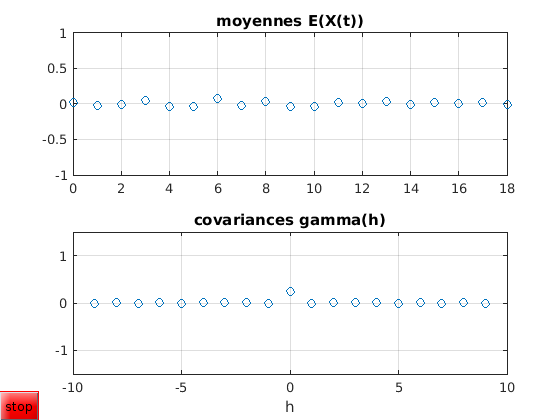
\includegraphics[width=8cm]{1-1.png}
    \caption{Bruit Blanc}
\end{figure}

$M_{W}=0$ pour un bruit blanc $\\$
$cov(W(n_{1}),W(n_{2}))=\mathbb{E}[W(n_{1})^{2}W(n_{2})^{2}] = \sigma^{2}\delta(n_{1},n_{2})$

$\\$

\subsection{Processus AR1 causal défini par $H(z)=\frac{1}{1-az^{-1}}$}

\begin{figure}[!h]
    \center
    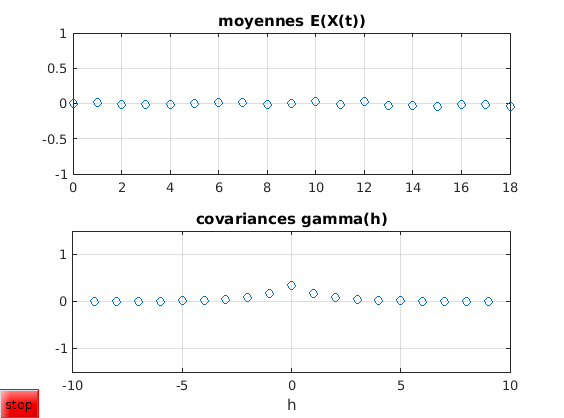
\includegraphics[width=7cm]{1-2.png}
    \caption{Processus AR1 causal}
\end{figure}

Après calcul on trouve la relation $Y(n) = \sum_{i=0}^na^{i}W(n-i)$ $\\$
La moyenne du processus est donc trivialement nulle comme somme de moyennes nulles de bruits blancs. $\\$
La covariance : $cov(X(n_{1}),X(n_{2}))= \frac{1-a^{n_{1}}}{1-a^{n_{1}-n_{2}}}$


\subsection{Processus sinusoidal $X(n)=b\cos(2\pi\nu_{0}n+\phi)$ où $\nu_{0} \in [0,0.5[, \phi$ étant une v.a. uniforme sur $[0,2]$ indépendante des $W(n)$}

\begin{figure}[!h]
    \center
    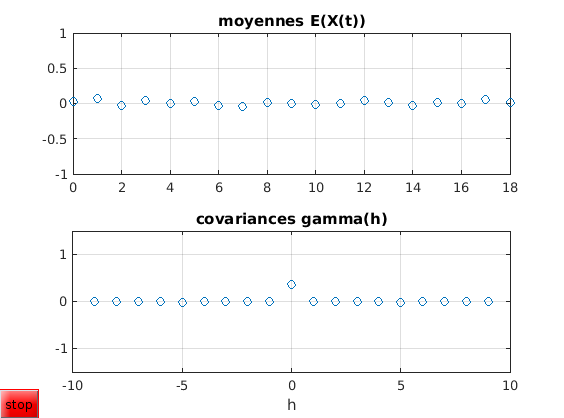
\includegraphics[width=7cm]{1-3.png}
    \caption{Processus sinusoïdal}
\end{figure}

$M_{X}(n)=b\int_{0}^{2\pi} \cos(2\pi\nu_{0}n+\phi)\frac{\deriv\phi}{2\pi} + 0 = 0$ $\\$
Il vient par calcul que $cov(X(n_{1}),X(n_{2}))=0$

\section{Estimation de la densité spectrale de puissance, périodogramme}

\subsection{Expression de $I_{X}(e^{2i\pi\nu})$ en fonction de la TFTD de $X$}

\begin{align*}
I_{X}(e^{2i\pi\nu})  &=\sum_{p=-N+1}^{N-1}\frac{1}{N}\sum_{i=1}^{N-p}X_{i+p}\bar{X_{i}}e^{-2i\pi\nu p} \\
&= \frac{1}{N}\sum_{p=-N+1}^{N-1}\sum_{i=1}^{N-p}X_{i+p}\bar{X_{i}}e^{-2i\pi\nu p} 
\end{align*}

On fait un changement de variable :
 \[\left\{
  \begin{array}{rcr}
    p & = & n_{2}-n_{1} \\
    i & = & n_{1} \\
  \end{array}
\right.\]

\begin{align*}
I_{X}(e^{2i\pi\nu})  &=\frac{1}{N}\sum_{p=-N+1}^{N-1}\sum_{i=max(0,-p)}^{N-1+min(0,-p)}X_{n_{2}}\bar{X_{n_{1}}}e^{-2i\pi\nu p} \\
&=\frac{1}{N}\sum_{n_{1}=0}^{N-1}\sum_{n_{2}=0}^{N-1}X_{n_{2}}\bar{X_{n_{1}}}e^{-2i\pi\nu (n_{2}-n_{1})} \\
&=\frac{1}{N} \left( \sum_{n_{1}=0}^{N-1}\bar{X_{n_{1}}}e^{2i\pi\nu n_{1}}\right)\left(\sum_{n_{2}=0}^{N-1}X_{n_{2}}e^{-2i\pi\nu n_{2}}\right) \\
&=\frac{1}{N} \left(\overline{\sum_{n_{1}=0}^{N-1}X_{n_{1}}e^{2i\pi\nu n_{1}}}\right)\left(\sum_{n_{2}=0}^{N-1}X_{n_{2}}e^{-2i\pi\nu n_{2}}\right) \\
&=\frac{1}{N}|TFTD[X(n)]|^{2}
\end{align*}

\subsection{Algorithme de calcul de $I_{X}(e^{2i\pi\nu})$}

Le code suivant permet d'obtenir $I_{X}(e^{2i\pi\nu})$ à partir de la TFD en posant $\nu=\frac{k}{M}$ où $k\in[0,N-1]$ et $M\geq N$, on obtient également la variance :
\begin{lstlisting}
TFD = fft(X, m);
        IX = (1/n)*abs(TFD).^2 ; 

        Variance = var(IX);
\end{lstlisting}

Ensuite on teste le code pour les 3 processus de la partie 1 :


\begin{figure}[h!]
    \begin{minipage}[c]{.46\linewidth}
        \centering
        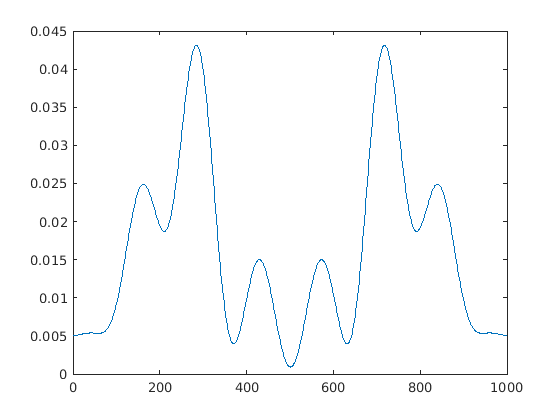
\includegraphics[width=7cm]{2-2.png}
        \caption{Bruit blanc}
    \end{minipage}
    \hfill%
    \begin{minipage}[c]{.46\linewidth}
        \centering
        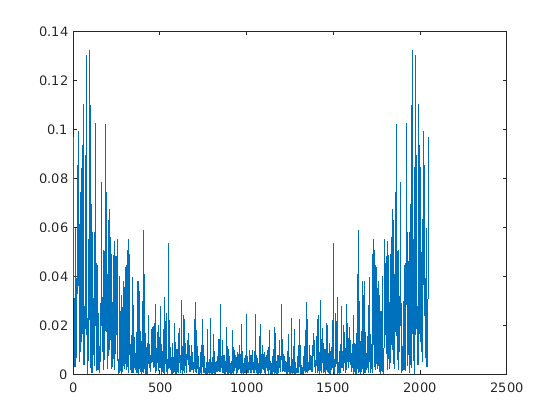
\includegraphics[width=7cm]{2-2-2}
        \caption{Processus AR1 causal}
    \end{minipage}
\end{figure}


\begin{figure}[!h]
    \center
    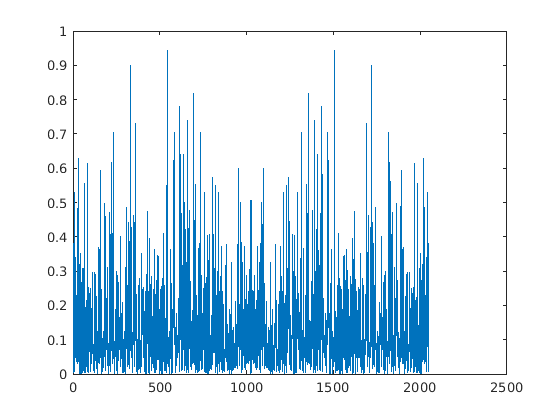
\includegraphics[width=7cm]{2-2-3.png}
    \caption{Processus sinusoïdal}
\end{figure}



\subsection{Calcul de la séquence des autocovariances estimées biaisées $R_{xx}(p)$ à partir de $I_{X}(e^{2i\pi\frac{k}{M}})$}

Le code suivant permet d'obtenir la séquence : 
\begin{lstlisting}

RXX = ifft(IX, m);
\end{lstlisting}

\subsection{variance du périodogramme d'un bruit blanc pour plusieurs horizons d'observation N}
On calcule la moyenne des variances sur 1000 répétitions en fonction de N.
\begin{figure}[!h]
    \center
    \includegraphics[width=7cm]{2-4.png}
    \caption{Moyenne des variances en échelle log2}
\end{figure}

\section{Filtrage des processus, modélisation AR de la parole}
\subsection{Equations de Yule-Walker}

\paragraph{Montrons que pour tout $k \leq 1$ on a $\mathbb{E}[X(n-k)W(n)]=0$ : }
$\\\\$
On prend $k \leq 1$ donc $X(n-k)$ et $W(n)$ sont indépendantes et $W$ est un bruit blanc , par suite : $\\$
\begin{align*}
\mathbb{E}[X(n-k)W(n)]&=\mathbb{E}[X(n-k)]\mathbb{E}[W(n)]  \ et  \ \mathbb{E}[W(n)]=0  \\
\end{align*}

Alors : 
\begin{align*}
 \mathbb{E}[X(n-k)W(n)]=0 \\
\end{align*}

\paragraph{On en déduit une relation entre les  $ R_{xx}(k) $ ... $ R_{xx}(k-p)$ pour $ k \geq 1 $ : }

\begin{align*}
X_{n}&=\sum_{m=1}^{p}a_{m}X_{n-m} + W_{n} \\
\mathbb{E}[X_{n}\bar{X_{n-k}}]&=\sum_{m=1}^{p}a_{m}\mathbb{E}[X_{n-m}\bar{X_{n-k}}] + \mathbb{E}[W_{n}\bar{X_{n-k}}] \\
\end{align*}

On pose $n_{1}=n-k$ $\\\\$
Or $\mathbb{E}[X_{n-m}\bar{X_{n-k}}]=\mathbb{E}[X_{n_{1}+k-m}\bar{X_{n_{1}}}]=R_{X}(k-m)$ et $\mathbb{E}[W_{n}\bar{X_{n-k}}]=0$ par la question précédente, il vient que :

\begin{align*}
\mathbb{E}[X_{n_{1}}\bar{X_{n_{1}-k}}]&=\sum_{m=1}^{p}a_{m}R_{X}(k-m)  \\
\end{align*}

Et 
\begin{align*}
\mathbb{E}[X_{n_{1}}\bar{X_{n_{1}-k}}]&=\mathbb{E}[X_{n+k}\bar{X_{n}}] \\
\end{align*}
Donc 
\begin{align*}
\mathbb{E}[X_{n+k}\bar{X_{n}}]&=\sum_{m=1}^{p}a_{m}R_{X}(k-m) \\
\end{align*}



On en déduit que :


\begin{align*}
%\frac{1}{N}\sum_{n=0}^{N+k-1}\bar{X_{n}}X_{n-k}&=\frac{1}{N}\sum_{n=0}^{N-k-1}X_{n}\bar{X_{n+k}} \\
\mathbb{E}[\hat{R}_{X}(k)]&=\frac{1}{N}\sum_{n=0}^{N-k-1}\mathbb{E}[\bar{X_{n}}X_{n+k}] \\
&=\frac{1}{N}\sum_{n=0}^{N-k-1}\left(\sum_{m=1}^{p}a_{m}R_{X}(k-m)\right) \\
&=\frac{N-k}{N}\sum_{m=1}^{p}a_{m}R_{X}(k-m) \\
\end{align*}

En passant la limite quand N tend vers l'infini dans les deux membres de l'égalité, on obtient finalement :

\begin{align*}
R_{X}(k)&=\sum_{m=1}^{p}a_{m}R_{X}(k-m) \\
\end{align*}

\paragraph{cas $k=0$}

\begin{align*}
\mathbb{E}[X_{n}W_{n}]&=\sum_{m=1}^{p}a_{m}\mathbb{E}[X_{n-m}W_{n}]+\mathbb{E}[W_{n}W_{n}] \\
\end{align*}

Or $\mathbb{E}[X_{n-m}W_{n}]=0$ car $X$ et $W$ sont indépendantes pusique $m \geq 1$ $\\$
Et $\mathbb{E}[W_{n}W_{n}]=\sigma^{2}$

\begin{align*}
%\frac{1}{N}\sum_{n=0}^{N+k-1}\bar{X_{n}}X_{n-k}&=\frac{1}{N}\sum_{n=0}^{N-k-1}X_{n}\bar{X_{n+k}} \\
\mathbb{E}[\hat{R}_{X}(0)]&=\frac{1}{N}\sum_{n=0}^{N-k-1}\mathbb{E}[\bar{X_{n}}X_{n}] \\
&=\frac{1}{N}\sum_{n=0}^{N-k-1}\left(\sum_{m=1}^{p}a_{m}R_{X}(-m)+\sigma^{2}\right) \\
&=\frac{N-k}{N}\left(\sum_{m=1}^{p}a_{m}R_{X}(k-m)+\sigma^{2}\right) \\
\end{align*}

En passant la limite quand N tend vers l'infini dans les deux membres de l'égalité, on obtient finalement :

\begin{align*}
R_{X}(0)&=\sum_{m=1}^{p}a_{m}R_{X}(-m)+\sigma^{2}\\
\end{align*}

Pour résumer, on a :

\[\left\{
  \begin{array}{lcl}
R_{X}(0)&=& \sum_{m=1}^{p}a_{m}R_{X}(-m)+\sigma^{2} \\
R_{X}(k)&=& \sum_{m=1}^{p}a_{m}R_{X}(k-m) \ \ \ \ \ pour \ k\geq 1\\  
  \end{array}
\right.\]



\paragraph{Forme matricielle du problème :}

Les rangs $k$ correspondent aux lignes de la matrice, il y en a donc $p+1$, les colonnes correspondent aux indices $i$ des $a_{i}$, il y en également p+1. Pour s'en convaincre on peut réécrire le système précédent :

\[\left\{
  \begin{array}{lcl}
R_{X}(0)-\sum_{m=1}^{p}a_{m}R_{X}(-m))&=& \sigma^{2} \\
R_{X}(k)-\sum_{m=1}^{p}a_{m}R_{X}(k-m)&=&0  \ \ \ \ \ pour \ k\geq 1\\    
  \end{array}
\right.\]

$\\$


$\left
(\begin{array}{cccc}
R_{X}(0) & -a_{1}R_{X}(-1) & \cdots & -a_{p}R_{X}(-p)\\
R_{X}(1) & -a_{1}R_{X}(0) & \cdots & -a_{p}R_{X}(1-p)\\
R_{X}(2) & -a_{1}R_{X}(1) & \cdots & -a_{p}R_{X}(2-p)\\
\vdots & \vdots & \vdots & \vdots\\
R_{X}(p) & -a_{1}R_{X}(p-1) & \cdots & -a_{p}R_{X}(0)
\end{array}\right)=[\sigma^{2}  \ 0 \ ... \ 0]^{T}
$

$\\\\$

$R=\left
(\begin{array}{cccc}
R_{X}(0) & R_{X}(-1) & \cdots & R_{X}(-p)\\
R_{X}(1) & R_{X}(0) & \cdots & R_{X}(1-p)\\
R_{X}(2) & R_{X}(1) & \cdots & R_{X}(2-p)\\
\vdots & \vdots & \vdots & \vdots\\
R_{X}(p) & R_{X}(p-1) & \cdots & R_{X}(0)
\end{array}\right)
$

$\\$

\begin{align*}
R\ [1 \ -a_{1} ... -a_{p}]^{T}=[\sigma^{2}  \ 0 \ ... \ 0]^{T} \\
\end{align*}
 


R est bien une matrice Toeplitz.


\subsection{Estimation}
\paragraph{Génération d'un processus AR-4 :}
$\\\\$
Le code suivant permet de générer un processus AR-4 en fontion d'un vecteur $a$ donné en entrée :

\begin{lstlisting}
function[R] = genAR(p, N, a)

    R = zeros(1, N);
    
    sigma = 1;
    
    W =  sigma.*randn(1,N);
    for n=1:N
       
        for i=1:min(n-1,p)
            R(n) = R(n) + a(i)*R(n-i);
            
        end
        
        R(n) = R(n) + W(n);
        
    end

end
\end{lstlisting}

\paragraph{Matrice Toeplitz estimée :}

$\\\\$
\begin{lstlisting}
p = 4;
N = 1000000;
NbRepet = 1000

for poi=1:NbRepet
    [X, phi] = genAR(p,N);

    Autocov = acovb(X);

    R = toeplitz(Autocov(1:p+1));
end
\end{lstlisting}

\paragraph{Résolution du système (1) : }
$\\$
\begin{align*}
\hat{R}\ [1 \ -a_{1} ... -a_{p}]^{T}&=[\sigma^{2}  \ 0 \ ... \ 0]^{T} \\
\hat{R}^{-1} \ \hat{R}\ [1 \ -a_{1} ... -a_{p}]^{T}&=\hat{R}^{-1} \ [\sigma^{2}  \ 0 \ ... \ 0]^{T} \\
[1 \ -a_{1} ... -a_{p}]^{T}&=\hat{R}^{-1} \ [\sigma^{2}  \ 0 \ ... \ 0]^{T} \\
[\frac{1}{\sigma^{2}} \ \frac{-a_{1}}{\sigma^{2}} ... \frac{-a_{p}}{\sigma^{2}}]^{T}&=\hat{R}^{-1} \ [1  \ 0 \ ... \ 0]^{T} \\
\end{align*}

donc $v=[\frac{1}{\sigma^{2}} \ \frac{-a_{1}}{\sigma^{2}} ... \frac{-a_{p}}{\sigma^{2}}]^{T}$

\paragraph{Comparaison :}

$\\\\$
On obtient une erreur quadratique moyenne de 0.2884 pour les valeurs estimées des coefficients du vecteur $a$ ainsi que pour $\sigma$.

\end{document}

